\documentclass[12pt]{article}
\usepackage{amsmath}
\usepackage{alltt}
\usepackage{amsfonts}
\usepackage{graphicx,psfrag,epsf}
\usepackage{enumerate}
\usepackage{amscd}
\usepackage{natbib}
\usepackage{tikz-cd}
\usepackage{adjustbox}
\usepackage{url} 

%\pdfminorversion=4
% NOTE: To produce blinded version, replace "0" with "1" below.
\newcommand{\blind}{1}

\newcommand{\R}{\mathbb{R}}
\newcommand{\E}{\text{E}}
\newcommand{\T}{\mathrm{T}}
\newcommand{\D}{\mathcal{D}}
\newcommand{\tauenv}{\hat{\tau}_{\text{env}}}
\newcommand{\tauhat}{\hat{\tau}}
\newcommand{\upenv}{\hat{\upsilon}_{\text{env}}}

\DeclareMathOperator{\Var}{Var}

% DON'T change margins - should be 1 inch all around.
%\addtolength{\oddsidemargin}{-.5in}%
%\addtolength{\evensidemargin}{-.5in}%
%\addtolength{\textwidth}{1in}%
%\addtolength{\textheight}{-.3in}%
%\addtolength{\topmargin}{-.8in}%

\title{Aster and envelopes}
\author{Daniel J. Eck}

\begin{document}

\maketitle

Aster models \citep*{geyer-aster} were developed for use in life history 
analyses \citep*{shaw-aster}. A specific application of aster models in life 
history analysis is the estimation of expected Darwinian fitness across 
covariates and trait values of interest where Darwinian fitness is the total 
offspring for a plant or animal over the course of its lifetime. The estimates 
of expected Darwinian fitness are plotted in a fitness landscape when 
covariates and trait values are continuous \citep*{shaw-fit-land, eck-evol}.

More formally, aster models \citep*{geyer-aster} are directed graphical models 
that satisfy the following five structural assumptions:
\begin{itemize}
{\setlength\itemindent{20pt}\item[A1.] The directed graph is acyclic.}
{\setlength\itemindent{20pt}\item[A2.] A node has, at most, one 
  predecessor node.}
{\setlength\itemindent{20pt}\item[A3.] The joint distribution is the product 
  of conditional distributions, one conditional distribution for each arrow in 
  the aster graph.}
{\setlength\itemindent{20pt}\item[A4.] Predecessor is sample size. }
{\setlength\itemindent{20pt}\item[A5.] Conditional distributions for arrows 
  are one-parameter exponential families. The exponential families across 
  arrows are not required to be the same. }
\end{itemize}
Assumptions A4 and A5 mean for an arrow $y_k \longrightarrow y_j$
that $y_j$ is the sum of independent and identically distributed random
variables from the exponential family for the arrow and there are $y_k$
terms in the sum where the sum of zero terms is zero \citep*{eck-asterenv}. 
The sum $y_j$ must be over discrete exponential families when $y_j$ is not a 
terminal node in the aster graph. These assumptions imply that the joint 
distribution of the aster model is an exponential family 
\citep*[Section 2.3]{geyer-aster}. In life history analyses, terminal nodes 
of the aster model correspond to offspring counts, while intermediate nodes 
represent important life stages in the plant or animal's life leading up to 
reproduction. 

The aster model is a ``generalized" generalized linear regression model (glm)
for one parameter exponential families. All one parameter glms can be 
represented as an aster model. However, in aster, only the canonical link 
function can be used or the joint distribution of the aster model will cease 
to be an exponential family and inferential abilities of the aster model will 
be lost.


\begin{figure}[t!]
  \begin{center}
    \setlength{\unitlength}{0.38 in}
    \thicklines
    \begin{picture}(10.3,2.8)(-0.1,-2.3)
      \put(0,0){\makebox(0,0){$1_{\hphantom{0}}$}}
      \put(1,0){\makebox(0,0){$A_1$}}
      \put(2,0){\makebox(0,0){$A_2$}}
      \put(3,0){\makebox(0,0){$A_3$}}
      \put(4,0){\makebox(0,0){$A_4$}}
      \put(5,0){\makebox(0,0){$A_5$}}
      \put(6,0){\makebox(0,0){$A_6$}}
      \put(7,0){\makebox(0,0){$A_7$}}
      \put(8,0){\makebox(0,0){$A_8$}}
      \put(9,0){\makebox(0,0){$A_9$}}
      \put(10,0){\makebox(0,0){$A_{10}$}}
      \multiput(0.35,0)(1,0){10}{\vector(1,0){0.3}}
      \put(1,-1){\makebox(0,0){$B_1$}}
      \put(2,-1){\makebox(0,0){$B_2$}}
      \put(3,-1){\makebox(0,0){$B_3$}}
      \put(4,-1){\makebox(0,0){$B_4$}}
      \put(5,-1){\makebox(0,0){$B_5$}}
      \put(6,-1){\makebox(0,0){$B_6$}}
      \put(7,-1){\makebox(0,0){$B_7$}}
      \put(8,-1){\makebox(0,0){$B_8$}}
      \put(9,-1){\makebox(0,0){$B_9$}}
      \put(10,-1){\makebox(0,0){$B_{10}$}}
      \multiput(1,-0.25)(1,0){10}{\vector(0,-1){0.5}}
      \put(1,-2){\makebox(0,0){$C_1$}}
      \put(2,-2){\makebox(0,0){$C_2$}}
      \put(3,-2){\makebox(0,0){$C_3$}}
      \put(4,-2){\makebox(0,0){$C_4$}}
      \put(5,-2){\makebox(0,0){$C_5$}}
      \put(6,-2){\makebox(0,0){$C_6$}}
      \put(7,-2){\makebox(0,0){$C_7$}}
      \put(8,-2){\makebox(0,0){$C_8$}}
      \put(9,-2){\makebox(0,0){$C_9$}}
      \put(10,-2){\makebox(0,0){$C_{10}$}}
      \multiput(1,-1.25)(1,0){10}{\vector(0,-1){0.5}}
    \end{picture}
  \end{center}  
  \caption{Graphical structure of the aster model for the simulated data in 
  \citet*[Example 1]{eck-asterenv}. The top layer corresponds to survival; 
  these random variables are Bernoulli. The middle layer corresponds to 
  whether or not an individual reproduced; these random variables are also 
  Bernoulli. The bottom layer corresponds to offspring count; these random 
  variables are zero-truncated Poisson.}
  \label{ex1-graph}
\end{figure}


The log likelihood for the aster model in canonical form is
$$ 
  l(\beta) = \langle M^TY, \beta \rangle - c(a + M\beta)
$$  
with canonical statistic $M^TY$, $Y \in \R^m$ is the vector of responses 
consisting of one component for every node in the graph for every individual 
in the study, $M$ is the model matrix assumed to have full column rank, $a$ is 
a known offset vector, and $\beta$ is the aster submodel canonical parameter 
vector. 

One key difference between aster models and other methods in which envelope 
methodology is applied is that inference with respect to $\beta$ is not 
desired. This is due in part to the fact that $M\beta_1$ and $M\beta_2$ can 
have the same value despite $\beta_1 \neq \beta_2$. Envelope methodology is 
not invariant to this type of non-uniqueness. To incorporate envelope 
methodology into the aster modeling framework, we focus on the aster submodel 
mean-vector parameter $\tau = E(M^TY)$ which is a well-defined quantity in 
aster modeling \citep*{geyer-phil, eck-asterenv}.

%The aster model, being a regular full exponential family, allows us to 
%conveniently obtain the maximum likelihood estimator for $\beta$. Then $\tau$ 
%is estimated by differentiation. We see that
%$$
% \tau = \nabla_{\beta} c(a + M\beta) = M^T \nabla c(\varphi) 
%      = \E(M^TY) = M^T\mu
%$$ 
%and the MLE of $\tau$, denoted $\hat{\tau}$, is $M^TY$. 

We now go through some details of \citet*[Example 1]{eck-asterenv} to explore 
how envelope methodology fits within the context of aster modeling.

%A population of 3000 organisms was simulated to form the dataset used in this 
%aster analysis. We generated data according to a known reducing subspace and show that our methods recover the true indices of the reducing subspace that generated the data. These data are generated according to the graphical structure appearing in panel C of Figure~\ref{Fig:graphs}. There are two covariates $(z_1,z_2)$ associated with Darwinian fitness and the aster model selected by the LRT is a full quadratic model with respect to these covariates. A full aster analysis of data of the same kind and its construction can be seen in \cite{geyer-land-tech}.

%In our example we consider the partial envelope approach. We partition $\tau$ into $(\gamma^T, \upsilon^T)^T$ where $\gamma \in \R^4$ are nuisance parameters and $\upsilon \in \R^5$ are relevant to the estimation of expected Darwinian fitness. Here, $\upsilon \in \R^5$ because our model is full quadratic in $z_1$ and $z_2$. The true reducing subspace is the space spanned by the first and fourth eigenvectors of the covariance matrix of the parameters of interest estimated from the original data. We begin by considering envelope estimators constructed using the 1D algorithm. AIC, BIC, and the LRT at $\alpha = 0.05$ all select $u = 5$. This selection is equivalent to supposing that no non-trivial envelope structure is present and one should proceed with the aster analysis using maximum likelihood estimation and conventional \texttt{aster} software. The parametric bootstrap procedure discussed in Figure~\ref{Fig:algoone} is not interesting in this case. We now consider envelope estimators constructed from reducing subspaces.

%AIC, BIC, and the LRT at $\alpha = 0.05$ all select a reducing subspace that is the sum of more eigenspaces than the true reducing subspace but fewer eigenspaces than the full space. There is also some disagreement between the model selection criteria. BIC and the LRT at $\alpha = 0.05$ select the reducing subspace that is the sum of the first, fourth, and fifth eigenspaces of $\widehat{\Sigma}_{\upsilon,\upsilon}$, denoted $\widehat{G}_1$. AIC selects the reducing subspace that is the sum of every eigenspace of $\widehat{\Sigma}_{\upsilon,\upsilon}$ except for the third eigenspace, denoted $\widehat{G}_2$. The parametric bootstrap algorithm discussed in Figure~\ref{Fig:algotwo} is used to estimate the asymptotic variability of $g(\hat{\tau}_{\text{env}})$ using the reducing subspace $\widehat{G}_1$. The results are seen in Table \ref{Tab5:target.env} for selected output. Table~\ref{Tab5:target.env} shows points that yield high values of estimated expected Darwinian fitness. The first two columns display the sample envelope estimator of expected Darwinian fitness and its bootstrapped standard error. The MLE of expected Darwinian fitness and its bootstrapped standard error are displayed in the third and fourth columns respectively. The ratios of bootstrapped standard errors for $g(\hat{\tau}_{\text{MLE}})$ to $g(\hat{\tau}_{\text{env}})$ are displayed in the final column. We can see that all of the ratios are greater than 1 which indicates that the envelope estimator of expected Darwinian fitness is less variable than the maximum likelihood estimator.

The dataset in this example is formed by generating data for 3000 organisms 
progressing through the lifecycle depicted in Figure~\ref{ex1-graph}. There 
is a known true envelope space in this example and it was shown that envelope 
methods in \citet*{eck-asterenv} find useful variance reduction at no cost to 
consistency. Darwinian fitness for this example is $\sum_{i=1}^{10}C_i$. There 
are two covariates $(z_1,z_2)$ associated with Darwinian fitness and the aster 
model used in this analysis supposes that expected Darwinian fitness is a full 
quadratic model in $z_1$ and $z_2$.

Partial envelope estimation is used in this example. The aster submodel 
mean-value parameter vector $\tau$ is partitioned into 
$(\gamma^T, \upsilon^T)^T$ where $\gamma \in \R^4$ are nuisance parameters and 
$\upsilon \in \R^5$ are relevant to the estimation of expected 
Darwinian fitness. Here, $\upsilon \in \R^5$ because our model is full 
quadratic in $z_1$ and $z_2$. We then estimate $\upsilon$ using both maximum 
likelihood estimation (the standard in aster) and envelope estimation. We use 
a weighted envelope estimator and a parametric bootstrap procedure suggested 
by \citet*{efron} to assess its variability. For more details, see 
\citet*{eck-asterenv}. 

The contour plots of the ratios of estimated standard errors for estimated 
expected Darwinian fitness are displayed in Figure~\ref{ex1-plots}. The 
contours show that the envelope estimator of expected Darwinian fitness is 
less variable than the maximum likelihood estimator for the majority of the 
observed data. Most importantly, we see efficiency gains at the values of 
$z_1$ and $z_2$ that maximize estimated expected Darwinian fitness.

One consequence of this example is that lower variability in estimation, 
resulting from the incorporation of envelope methodology, allows researchers 
in life history analysis to narrow their search for candidate trait values and 
covariates associated with interesting aspects of expected Darwinian fitness. 
This is of importance in life history analysis 
\citep*{eck-evol, shaw-fit-land}. All estimates of expected Darwinian fitness 
have variability in estimation. As a result, there can be many trait values 
statistically indistinguishable from the trait value which maximizes expected 
Darwinian fitness. We can see that the combination of envelope methodology 
with aster models leads to a useful reduction in the number of traits that are 
statistically indistinguishable from the reported maximizer of estimated 
expected Darwinian fitness. When aster is used alone, there are 14 candidate 
maximizers of estimated expected Darwinian fitness as opposed to only 7 
candidate maximizers of estimated expected Darwinian fitness when using 
envelope methodology.

%AIC, BIC, and the LRT at $\alpha = 0.05$ all select a reducing subspace that is the sum of more eigenspaces than the true reducing subspace but fewer eigenspaces than the full space. There is also some disagreement between the model selection criteria. BIC and the LRT at $\alpha = 0.05$ select the reducing subspace that is the sum of the first, fourth, and fifth eigenspaces of $\widehat{\Sigma}_{\upsilon,\upsilon}$, denoted $\widehat{G}_1$. AIC selects the reducing subspace that is the sum of every eigenspace of $\widehat{\Sigma}_{\upsilon,\upsilon}$ except for the third eigenspace, denoted $\widehat{G}_2$. The parametric bootstrap algorithm discussed in Figure~\ref{Fig:algotwo} is used to estimate the asymptotic variability of $g(\hat{\tau}_{\text{env}})$ using the reducing subspace $\widehat{G}_1$. The results are seen in Table \ref{Tab5:target.env} for selected output. Table~\ref{Tab5:target.env} shows points that yield high values of estimated expected Darwinian fitness. The first two columns display the sample envelope estimator of expected Darwinian fitness and its bootstrapped standard error. The MLE of expected Darwinian fitness and its bootstrapped standard error are displayed in the third and fourth columns respectively. The ratios of bootstrapped standard errors for $g(\hat{\tau}_{\text{MLE}})$ to $g(\hat{\tau}_{\text{env}})$ are displayed in the final column. We can see that all of the ratios are greater than 1 which indicates that the envelope estimator of expected Darwinian fitness is less variable than the maximum likelihood estimator.


\begin{figure}[h!]
  \begin{center}
    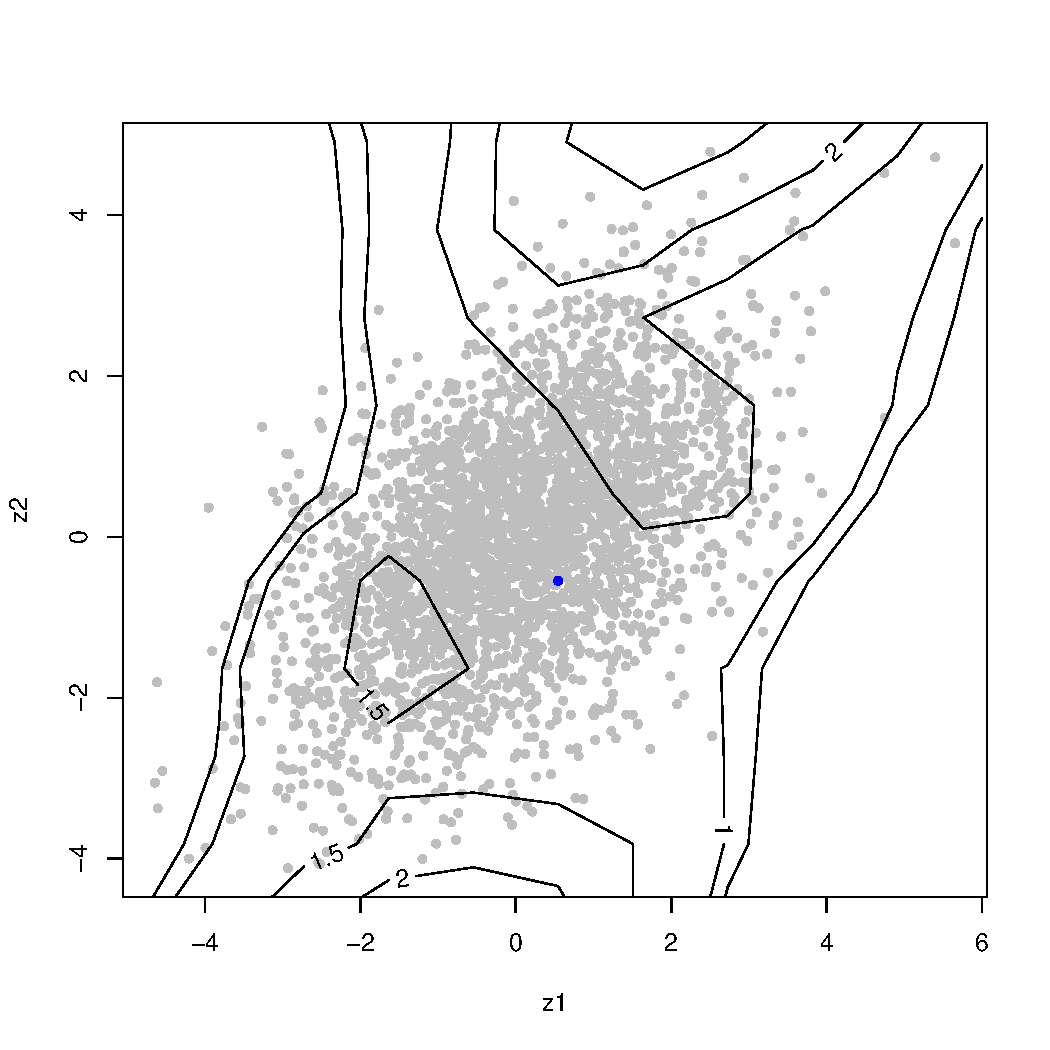
\includegraphics[width = 0.45\textwidth]{ex1-ratios-Efron-1.pdf}
    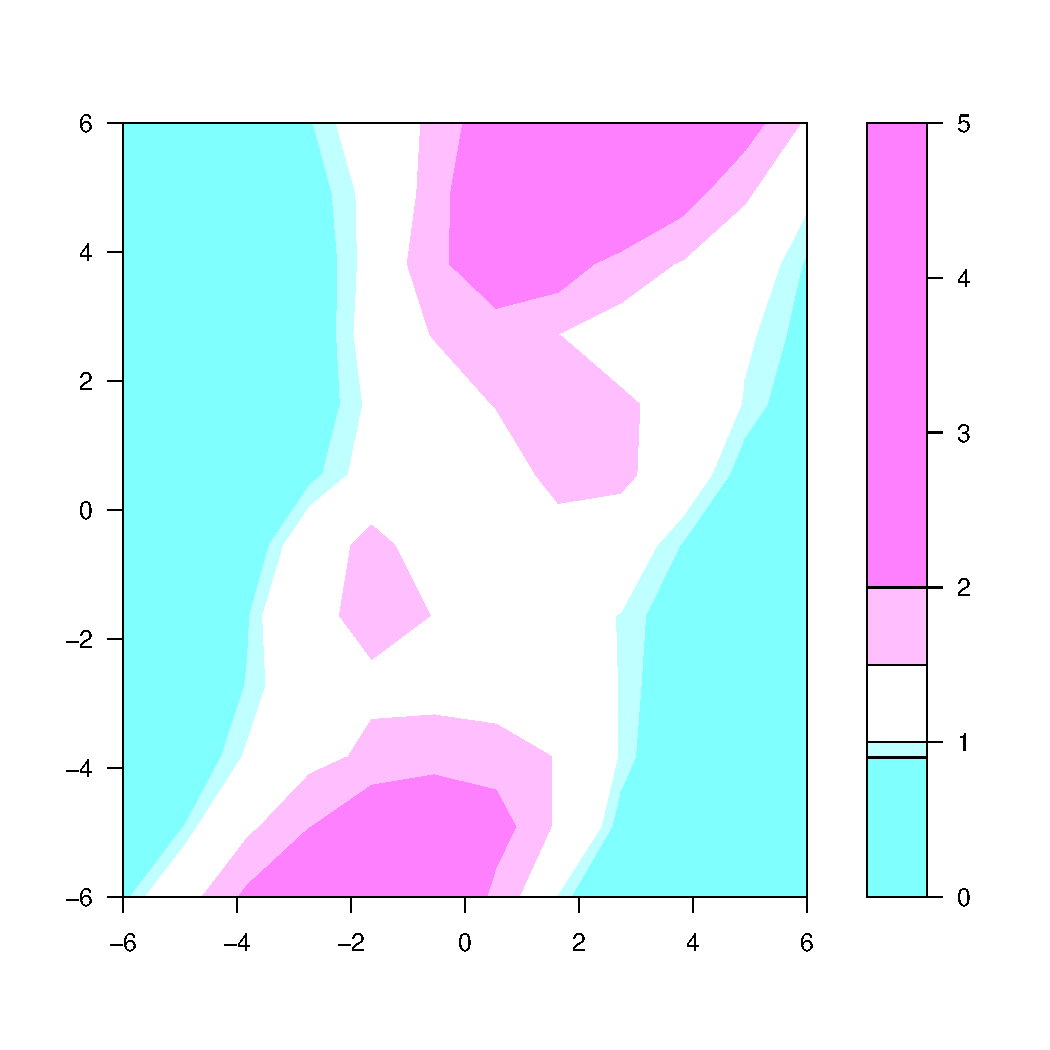
\includegraphics[width = 0.45\textwidth]{ex1-ratios-Efron-2.pdf}
  \end{center}
  \caption{Contour plots for the ratios of bootstrapped standard errors for 
  the model fit using the MLE to the ratios of bootstrapped standard errors 
  for the model fit using the envelope estimator. The point in blue 
  corresponds to the highest estimated expected Darwinian fitness value using 
  envelope methodology and the MLE. }
  \label{ex1-plots}
\end{figure}




\begin{thebibliography}{}

%\bibitem[Cook, et al.(2010)Cook, Li, and Chiaromonte]{cook}
%Cook, R.~D., Li, B., Chiaromonte, F. (2010).
%\newblock Envelope models for parsimonious and 
%efficient multivariate linear regression.
%\newblock \emph{Statistica Sinica}, \textbf{20}: 927-1010.


%\bibitem[Cook and Zhang(2015)Cook and Zhang]{cook3}
%Cook, R.~D., Zhang, X. (2015).
%\newblock Algorithms for Envelope Estimation.
%\newblock \emph{Journal of Computational and Graphical Statistics}, 
%Published online. \url{DOI:10.1080/10618600.2015.1029577}.


%\bibitem[Cook and Zhang(2015)Cook and Zhang]{cook2}
%Cook, R.~D., Zhang, X. (2015).
%\newblock Foundations for Envelope Models and Methods.
%\newblock \emph{JASA}, \textbf{110:510}: 599-611.


\bibitem[Eck, et al.(2015)Eck et al.]{eck-evol}
Eck, D.~J., Shaw, R., Geyer, C.~J., Kingsolver J.~G. (2015).
\newblock An Integrated Analysis of Phenotypic Selection on Insect Body Size
    and Development Time.
\newblock \emph{Evolution}, \textbf{69}: 2525-2532. 


\bibitem[Eck, et al.(2017)Eck, Geyer, and Cook]{eck-asterenv}
Eck, D.~J., Geyer, C.~J., and Cook, R.~D. (2017).
\newblock An Application of Envelope and Aster Models.
\newblock \emph{Submitted}.


%\bibitem[Eck(2015)]{envlp-package}
%Eck, D.~J. (2015).
%\newblock R package \texttt{envlpaster}, version 0.1-2.
%\newblock \url{http://cran.r-project.org/package=envlpaster}.


\bibitem[Eck, et. al.(2016)Eck, Geyer, and Cook]{ecktech}
Eck, D.~J., Geyer, C.~J., and Cook, R.~D. (2016).
\newblock Supporting Data Analysis for 
    ``An Application of Envelope Methodology and Aster Models."
\newblock \url{http://hdl.handle.net/11299/178384}.


\bibitem[Efron(2014)Efron]{efron}
Efron, B. (2014).
\newblock Estimation and Accuracy After Model Selection.
\newblock \emph{JASA}, \textbf{109:507}: 991-1007.


\bibitem[Geyer, et al.(2007)Geyer, Wagenius, and Shaw]{geyer-aster}
Geyer, C.~J., Wagenius, S., Shaw, R.~G. (2007).
\newblock Aster models for life history analysis.
\newblock \emph{Biometrika}, \textbf{94}: 415-426.


%\bibitem[Geyer and Shaw(2009)Geyer and Shaw]{geyer4}
%Geyer, C.~J. and Shaw, R.~G. (2009).
%\newblock Model Selection in Estimation of Fitness Landscapes. Technical Report
%No. 671. School of Statistics, University of Minnesota.
%\newblock \url{http://conservancy.umn.edu/handle/11299/56219.}


\bibitem[Geyer, C.~J.(2010)Geyer]{geyer-phil}
Geyer, C.~J. (2010).
\newblock A Philosophical Look at Aster Models. Technical Report
No. 676. School of Statistics, University of Minnesota.
\newblock \url{http://purl.umn.edu/57163.}


%\bibitem[Geyer(2010)]{aster2-package}
%Geyer, C.~J. (2010).
%\newblock R package aster2 (Aster Models), version 0.1.
%\newblock \url{http://cran.r-project.org/package=aster2}.


%\bibitem[Geyer(2014)]{aster-package}
%Geyer, C.~J. (2014).
%\newblock R package \texttt{aster} (Aster Models), version 0.8-30.
%\newblock \url{http://cran.r-project.org}.


%\bibitem[Lande and Arnold(1983)]{lande}
%Lande, R., Arnold, S. (1983).
%\newblock The measurement of selection on correlated characters.
%\newblock \emph{Evolution}, \textbf{37}: 1210-1226.


\bibitem[Shaw, et al.(2008)Shaw, Geyer, Wagenius, Hangelbroek, and Etterson]{shaw-aster}
Shaw, R.~G., Geyer, C.~J., Wagenius, S., Hangelbroek, H., and Etterson, J.~R. (2008).
\newblock Unifying life-history analyses for 
inference of fitness and population growth.
\newblock \emph{The American Naturalist}, \textbf{172}: E35-E47.


\bibitem[Shaw, et al.(2010)Shaw and Geyer]{shaw-fit-land}
Shaw, R.~G., Geyer, C.~J. (2010).
\newblock Inferring fitness landscapes.
\newblock \emph{Evolution}, \textbf{64}: 2510-2520.

\end{thebibliography}

\end{document}



